\documentclass[border=10pt]{standalone}
\usepackage{tikz}
\usetikzlibrary{arrows.meta, calc}

\begin{document}
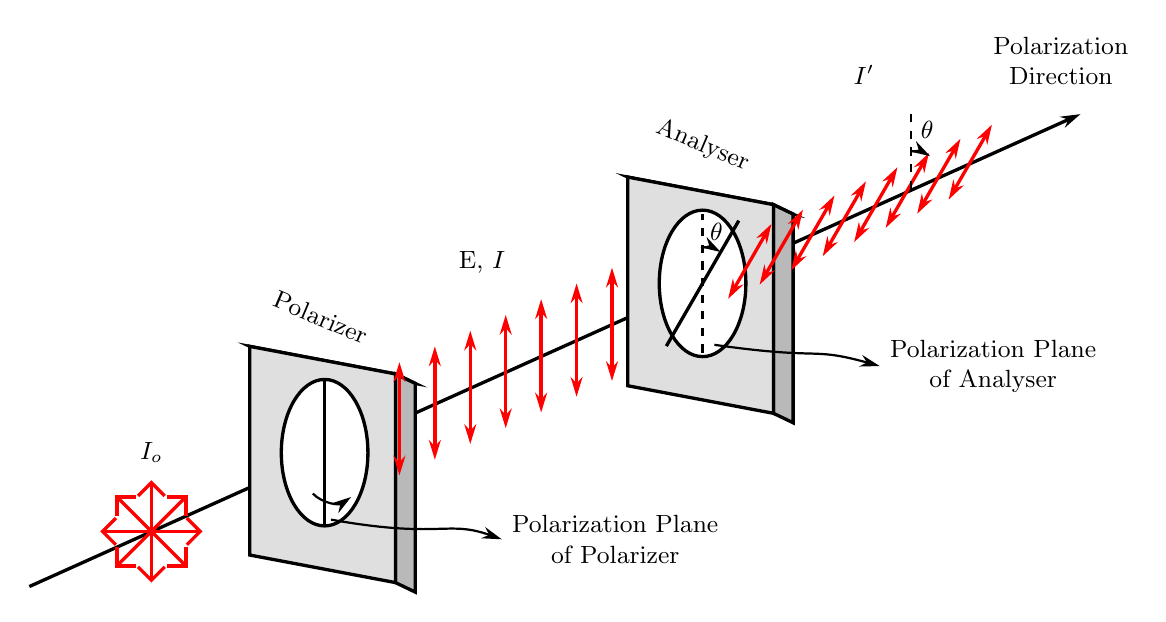
\begin{tikzpicture}[
    font=\small,
    >={Stealth[length=2.5mm, width=1.5mm]}
]
    % Define angle and coordinates for the oblique perspective
    \def\th{30} % Angle theta
    \coordinate (P1) at (4.2,1.85); % Polarizer center
    \coordinate (P2) at (9.0,4.00); % Analyzer center

    % Main beam path in oblique perspective
    \draw[very thick, ->] (0.45,0.15) -- (13.8,6.15);

    % 1. Unpolarized Light
    \coordinate (U) at (2.0,0.85);
    \node[above=0.75cm] at (U) {$I_o$};
    \foreach \angle in {0,45,...,315} {
        \draw[-{Straight Barb[length=1.7mm]}, red, very thick] (U) -- ++(\angle:0.65);
    }

    % 2. Polarizer: projected 3D plate
    \node[rotate=-23] at ($(P1)+(-0.05,1.72)$) {Polarizer};
    \filldraw[fill=gray!50, draw=black, very thick]
        ($(P1)+(-0.95,1.35)$) -- ($(P1)+(-0.70,1.23)$) -- ($(P1)+(1.15,0.88)$) -- ($(P1)+(0.90,1.00)$) -- cycle;
    \filldraw[fill=gray!55, draw=black, very thick]
        ($(P1)+(0.90,1.00)$) -- ($(P1)+(1.15,0.88)$) -- ($(P1)+(1.15,-1.77)$) -- ($(P1)+(0.90,-1.65)$) -- cycle;
    \filldraw[fill=gray!25, draw=black, very thick]
        ($(P1)+(-0.95,-1.30)$) -- ($(P1)+(0.90,-1.65)$) -- ($(P1)+(0.90,1.00)$) -- ($(P1)+(-0.95,1.35)$) -- cycle;
    % Aperture and axis
    \draw[fill=white, very thick] (P1) ellipse [x radius=0.55, y radius=0.93];
    \draw[very thick] ($(P1)+(0,-0.92)$) -- ($(P1)+(0,0.92)$);
    \draw[->, thick] ($(P1)+(-0.15,-0.52)$) arc (-135:-55:0.38);
    % Label for polarization plane
    \draw[->, thick]
        ($(P1)+(0.08,-0.85)$) .. controls +(1.4,-0.25) and +(-0.7,0.25) ..
        ($(P1)+(2.25,-1.10)$) node[right, align=center] {Polarization Plane\\of Polarizer};

    % 3. Vertically Polarized Light
    \node[above=0.95cm] at (6.2,3.05) {E, $I$};
    \foreach \x/\y in {5.15/2.28,5.60/2.48,6.05/2.68,6.50/2.88,6.95/3.08,7.40/3.28,7.85/3.48,8.30/3.68,8.65/3.84} {
        \draw[<->, red, very thick] (\x,\y-0.72) -- (\x,\y+0.72);
    }

    % 4. Analyser: projected 3D plate
    \node[rotate=-23] at ($(P2)+(0.00,1.75)$) {Analyser};
    \filldraw[fill=gray!50, draw=black, very thick]
        ($(P2)+(-0.95,1.35)$) -- ($(P2)+(-0.70,1.23)$) -- ($(P2)+(1.15,0.88)$) -- ($(P2)+(0.90,1.00)$) -- cycle;
    \filldraw[fill=gray!55, draw=black, very thick]
        ($(P2)+(0.90,1.00)$) -- ($(P2)+(1.15,0.88)$) -- ($(P2)+(1.15,-1.77)$) -- ($(P2)+(0.90,-1.65)$) -- cycle;
    \filldraw[fill=gray!25, draw=black, very thick]
        ($(P2)+(-0.95,-1.30)$) -- ($(P2)+(0.90,-1.65)$) -- ($(P2)+(0.90,1.00)$) -- ($(P2)+(-0.95,1.35)$) -- cycle;
    % Aperture and axis
    \draw[fill=white, very thick] (P2) ellipse [x radius=0.55, y radius=0.93];
    \draw[very thick] ($(P2)+(240:0.92)$) -- ($(P2)+(60:0.92)$);
    % Angle annotation on analyser
    \draw[dashed, thick] ($(P2)+(0,-0.88)$) -- ($(P2)+(0,0.88)$);
    \draw[->, thick] ($(P2)+(90:0.46)$) arc (90:60:0.46);
    \node at ($(P2)+(75:0.68)$) {$\theta$};
    % Label for polarization plane
    \draw[->, thick]
        ($(P2)+(0.15,-0.78)$) .. controls +(1.4,-0.20) and +(-0.9,0.25) ..
        ($(P2)+(2.25,-1.05)$) node[right, align=center] {Polarization Plane\\of Analyser};

    % 5. Final Polarized Light
    \node[above=0.95cm] at (11.05,5.45) {$I'$};
    \foreach \x/\y in {9.60/4.28,10.00/4.46,10.40/4.64,10.80/4.82,11.20/5.00,11.60/5.18,12.00/5.36,12.40/5.54} {
        \draw[<->, red, very thick, rotate around={-30:(\x,\y)}] (\x,\y-0.55) -- (\x,\y+0.55);
    }

    % 6. Final direction and angle
    \node[above=0.35cm, align=center] at (13.55,6.05) {Polarization\\Direction};
    \coordinate (A) at (11.65,5.20);
    \draw[dashed, thick] (A) -- ++(0,1.00);
    \draw[->, thick] ($(A)+(90:0.48)$) arc (90:60:0.48);
    \node at ($(A)+(75:0.78)$) {$\theta$};

\end{tikzpicture}
\end{document}
